\RequirePackage[T1]{fontenc}
\documentclass[conference,10pt]{IEEEtran}
\usepackage{amsmath,amssymb,booktabs,graphicx,url,array}
\usepackage{tikz}
\usetikzlibrary{arrows.meta,calc}
\usepackage[hidelinks]{hyperref}
\hypersetup{pdftitle={Deadline-Constrained Recovery and Cancellation in LoRa Mesh Networks},pdfauthor={},pdfsubject={Anonymous review manuscript},pdfkeywords={LoRa, mesh networks, routing recovery, simulation}}
\title{Deadline-Constrained Recovery and Cancellation in LoRa Mesh Networks}
\author{Anonymous authors}
\begin{document}
\maketitle
\begin{abstract}
Timely confirmation in a LoRa mesh requires both delivery of an application
message and return of its acknowledgment before a deadline. Reusing a
known route limits forwarding, but an unconfirmed attempt leaves the
source uncertain whether to repeat or broaden dissemination. MeshEcho-CPR
combines local deadline admission, at most one same-path repeat and one
recovery flood, and ACK-driven cancellation of uncommitted relay copies.
It separates message confirmation from shared route updates to preserve
newer evidence under concurrent flows. We evaluate the fixed controller
with three behavioral comparators and three component controls in 760
prespecified runs using 20 paired seeds per condition. Recovery has
opposite effects across two stress settings. With prescribed link
disruption, full CPR raises timely confirmation by 8.32 percentage points
over its no-recovery control (descriptive 95\% interval 4.90--11.63), at a
geometric mean airtime ratio of 1.27. Under higher traffic contention, it
reduces confirmation by 15.99 points (interval $-19.41$ to $-12.64$), at
an airtime ratio of 1.66. ACK cancellation reduces airtime in both settings,
while its confirmation effect is uncertain under contention. Physical
event accounting and exposed-route reconstruction retain unsuccessful
flows and identify where recovery actually runs. The results establish a
conditional trade-off in the declared simulator, motivating contention-aware
recovery admission; they do not establish product-firmware superiority or
hardware performance.
\end{abstract}
\begin{IEEEkeywords}
LoRa, mesh networks, routing recovery, relay cancellation, reproducible simulation
\end{IEEEkeywords}

\section{Introduction}
\label{sec:introduction}

LoRa's long frames make mesh reliability sensitive to airtime,
radio configuration, and message length~\cite{augustin2016study,bor2016scale}.
A delivered message is not necessarily a confirmed transaction: a valid
ACK must also reach the source before the deadline. Forward delivery
and reverse confirmation therefore need separate measurements.

Reusing a known route confines forwarding. Missing confirmation, however,
does not identify whether DATA or ACK was lost, a relay was busy, or the
route failed. Repetition may overcome a transient loss; broader
forwarding may find another path. Either can instead add contention.
A recovery policy must bound additional work, admit it against remaining
time, and define when feedback can still cancel a queued transmission.

MeshEcho-CPR addresses these decisions with a finite controller. An
ACK-confirmed route is tried first when locally feasible; a routed flow
can then repeat once and attempt one recovery flood. A flow initially
served by a flood has neither later stage. A matching ACK can cancel a
relay copy only before that copy commits to the radio schedule. The source
also distinguishes a live message's confirmation from shared cache
evidence, because concurrent messages can confirm or invalidate routes
in a different order from their creation.

The research question is when this combination changes the trade-off
between timely source confirmation and physical transmit airtime, and
which component causes the change. Source routing, finite retries,
flooding, and ACK-assisted coordination have established antecedents
\cite{johnson1996dsr,liu2004truncated,biswas2005exor}. The contribution
here is a precise interaction of these mechanisms and an auditable
evaluation of its conditions of benefit and failure. A generic
retry-followed-by-flood sequence is not claimed as new.

We provide an executable-policy specification with
finite source-stage bounds, explicit state limits, and a defined
cancellation boundary. Our measurements retain every
scheduled flow and every physical transmission, plus clean controls for
the repeat, recovery, and ACK-cancellation components. A frozen 760-run
study with 20 paired seeds per condition exposes both the benefit of
recovery under path disruption and its substantial confirmation penalty
under higher traffic contention. The recovery control changes timely
confirmation in opposite directions: $+8.32$ percentage points in the
disrupted setting and $-15.99$ points in the contention setting. This
reversal, rather than a universal efficiency claim, is the principal
empirical finding.
The comparison concerns MeshEcho-CPR, legacy MeshEcho, Meshtastic-like,
and MeshCore-like behavioral models. The last two omit documented
product mechanisms; their results cannot establish performance superiority
over official firmware.

\section{Related Work}
\label{sec:related}

LoRa capacity depends on airtime, radio configuration, timing, and
interference~\cite{bor2016scale,georgiou2017scale}. LoRaWAN studies also
distinguish received DATA from confirmed communication because ACK traffic
consumes constrained resources~\cite{vandenabeele2017scalability}.
Collision/capture experiments and ns-3 modeling motivate explicit reception
and interference treatment~\cite{rahmadhani2018concurrent,to2018lorans3}.
These studies do not calibrate the present simulator: inter-SF interference
and multi-interferer capture introduce further effects
\cite{croce2018orthogonality,heusse2023capacity}, and single-gateway results
do not establish multi-hop mesh performance.

Multi-hop LoRa research spans distinct relay/router architectures and
routing, access, and energy objectives
\cite{cotrim2020lorawanmesh,wong2024multihop}. Smart-Hop uses
spreading-factor-dependent range in a low-latency multi-hop design
\cite{ahmar2022smarthop}, while MLoRa targets economical coverage and
balanced energy use~\cite{feng2022cost}. Other approaches use SF clustering
to balance airtime~\cite{zhu2019improving} or time-on-air metrics in
distance-vector routing~\cite{pueyo2024minimalistic}. An ESP32 mesh library
and LoRaHop provide implementation evidence for proactive routing and
bidirectional LoRaWAN relaying, respectively
\cite{sole2022implementation,tian2023lorahop}. Their architectures and
hardware evidence cannot be treated as same-condition CPR baselines.

Source-route discovery and reuse are established by DSR
\cite{johnson1996dsr}, and finite ARQ exposes a delay--reliability trade-off
\cite{liu2004truncated}. Forward DATA and reverse ACK reception jointly
enter ETX's link cost~\cite{decouto2003etx}. Bursty low-power wireless
reception~\cite{srinivasan2008beta} further cautions against treating retry
outcomes as independent. CPR uses missing confirmation and local time
budgets; it does not implement an ETX estimator or derive reliability by
multiplying independent stage-success probabilities. Common-random-number
methods motivate shared-environment comparisons, although their variance
benefit is conditional on the system~\cite{glasserman1992crn}.

Redundant flooding creates contention and collision opportunities
\cite{ni1999broadcaststorm}. Trickle suppresses broadcasts after overhearing
consistent summaries~\cite{levis2004trickle}, while ExOR coordinates
opportunistic forwarding using acknowledgment information
\cite{biswas2005exor}. Official Meshtastic and MeshCore mechanisms likewise
include learned routes, retries, and flooding
\cite{meshtasticfirmware,meshcore}. Retry-to-flood recovery and ACK-assisted
suppression are therefore antecedents. CPR examines their specific
interaction with deadline admission, live-message confirmation, cache
evidence, and the point at which a relay send becomes committed.

The Meshtastic-like and MeshCore-like baselines are simplified behavioral
models. They omit official retry behavior; the former also omits next-hop
learning, while the latter uses RREQ/RREP rather than the documented
first-message DATA flood and delivery-report path learning. Comparisons
with these models cannot establish superiority over current product
firmware. Component controls isolate narrower CPR policy effects without
removing this external-fidelity limitation.

\section{System Model and Measurements}
\label{sec:model}

We study unicast application messages in a packet-level LoRa mesh model.
Each flow $i$ has unique identity, source $s_i$, destination $d_i$,
enqueue time $a_i$, and relative deadline $\Delta_i$:
\begin{equation}
D_i=a_i+\Delta_i.
\label{eq:deadline}
\end{equation}
The source observes its local flow state, cached path, radio queue,
configured PHY and timers, and decoded packets. Relays additionally use
received SNR and their configured role to schedule forwarding. No protocol
receives future faults, global reachability, or a destination-delivery
oracle. Offline graph diagnostics characterize the environment only.

Let $t_i^{D}$ be the first eligible destination reception and $t_i^{A}$
the first accepted source ACK; missing observations have time infinity.
For all $N$ scheduled flows, timely delivery and confirmation are
\begin{equation}
P_D=\frac{1}{N}\sum_i\mathbf{1}[t_i^{D}\le D_i],\qquad
P_A=\frac{1}{N}\sum_i\mathbf{1}[t_i^{A}\le D_i].
\label{eq:outcomes}
\end{equation}
Capacity rejection, no-start flows, and deadline misses remain in $N$.
An overheard routed packet is eligible delivery only when the destination
is its designated next hop. Delivery without timely confirmation is an
outcome, not by itself a diagnosis of ACK-channel loss.

For a fixed generation-plus-drain cutoff $C$, charge every distinct physical
transmission $q$ starting at $t_q\le C$:
\begin{equation}
A=\sum_{q:t_q\le C}T(L_q),\qquad
C_D=\frac{A}{\sum_i\mathbf{1}[t_i^{D}\le D_i]}.
\label{eq:physical-cost}
\end{equation}
$T(L)$ is full-frame LoRa time on air, using the standard symbol and
payload-length calculation~\cite{augustin2016study}. All DATA, ACK,
discovery, duplicate, and recovery transmissions are charged. A frame
starting before the cutoff is charged in full even if it ends later.
$C_D$ is undefined with zero timely deliveries. Requests and cancellations
are separate events; neither is a physical transmission.

For CPR, a path carrying $n$ node identifiers, useful payload of $P$ bytes,
and optional stage marker $m$ has modeled lengths
\begin{equation}
\begin{aligned}
L_{D/F}(n,m)&=12+2n+P+\mathbf{1}[m\ne\varnothing],\\
L_A(n,m)&=12+2n+\mathbf{1}[m\ne\varnothing].
\end{aligned}
\label{eq:wire}
\end{equation}
The ten-byte common header plus path count/index fields and two-byte node
IDs define this custom encoding. CPR's request ID equals its flow ID and
adds no discovery-ID extension. Cache generations and confirmation revisions
are local state. These lengths do not reproduce official product framing,
encryption, or authentication overhead.

\section{MeshEcho-CPR}
\label{sec:cpr}

% Reproducible vector diagram. Logical order and schematic timing only;
% positions are not measured latency or drawn to time scale.
\begin{figure*}[t]
\centering
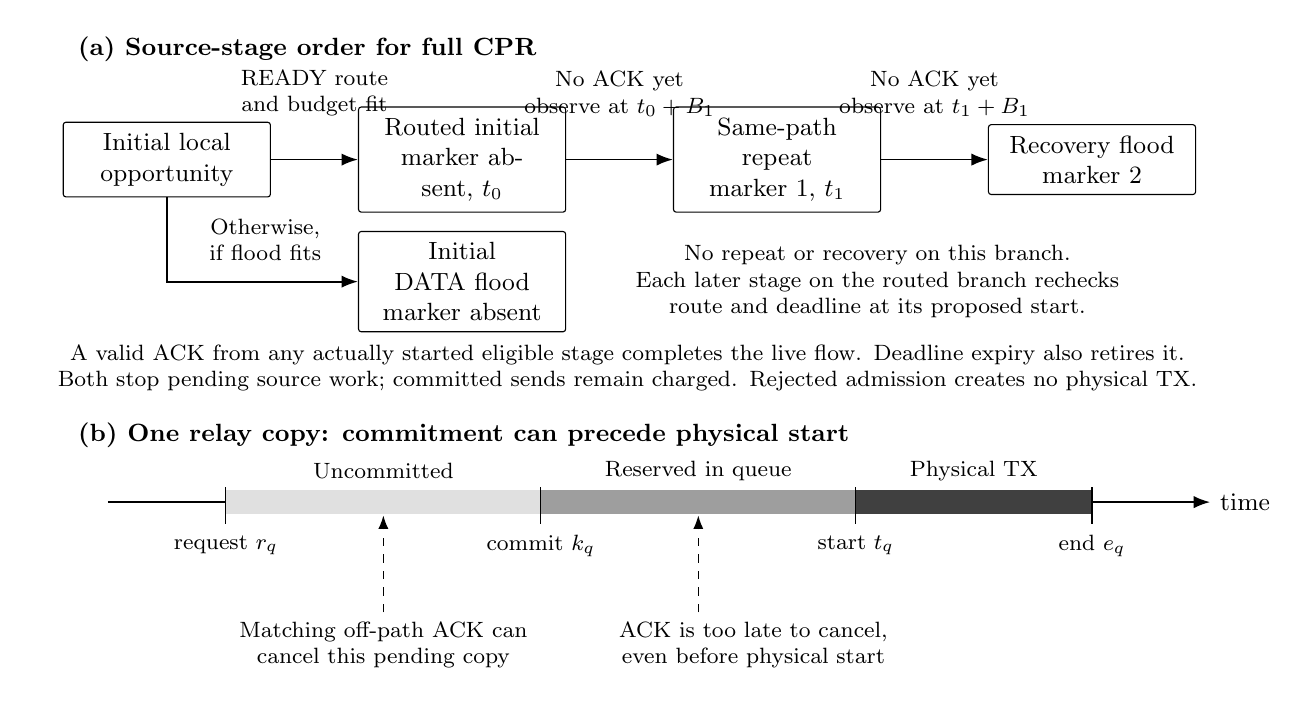
\begin{tikzpicture}[
  x=1cm,y=1cm,>=Latex,
  stage/.style={draw,rounded corners=1pt,align=center,font=\small,
    text width=2.35cm,minimum height=0.78cm,inner sep=4pt},
  annotation/.style={align=center,font=\footnotesize},
  flow/.style={->,line width=0.65pt}]

\node[anchor=west,font=\bfseries\small] at (0,3.5)
  {(a) Source-stage order for full CPR};
\node[stage] (select) at (1.25,2.1) {Initial local\\opportunity};
\node[stage] (initial) at (5,2.1) {Routed initial\\marker absent, $t_0$};
\node[stage] (repeat) at (9,2.1) {Same-path repeat\\marker 1, $t_1$};
\node[stage] (recovery) at (13,2.1) {Recovery flood\\marker 2};
\draw[flow] (select) -- node[annotation,above,yshift=12pt] {READY route\\and budget fit} (initial);
\draw[flow] (initial) -- node[annotation,above,yshift=12pt] {No ACK yet\\observe at $t_0+B_1$} (repeat);
\draw[flow] (repeat) -- node[annotation,above,yshift=12pt] {No ACK yet\\observe at $t_1+B_1$} (recovery);

\node[stage] (cold) at (5,0.55) {Initial DATA flood\\marker absent};
\draw[flow] (select.south) |- (cold.west);
\node[annotation] at (2.5,1.08) {Otherwise,\\if flood fits};
\node[annotation,anchor=west,text width=6.7cm] at (6.8,0.55)
  {No repeat or recovery on this branch.\\
   Each later stage on the routed branch rechecks route and deadline at its proposed start.};
\node[annotation,text width=15cm] at (7.1,-0.55)
  {A valid ACK from any actually started eligible stage completes the live flow.
   Deadline expiry also retires it.\\
   Both stop pending source work; committed sends remain charged.
   Rejected admission creates no physical TX.};

\node[anchor=west,font=\bfseries\small] at (0,-1.4)
  {(b) One relay copy: commitment can precede physical start};
\draw[->,line width=0.65pt] (0.5,-2.25) -- (14.5,-2.25) node[right,font=\small] {time};
\fill[black!12] (2,-2.1) rectangle (6,-2.4);
\fill[black!38] (6,-2.1) rectangle (10,-2.4);
\fill[black!75] (10,-2.1) rectangle (13,-2.4);
\foreach \x/\lab in {2/{request $r_q$},6/{commit $k_q$},10/{start $t_q$},13/{end $e_q$}} {
  \draw (\x,-2.06) -- (\x,-2.53);
  \node[annotation,below] at (\x,-2.55) {\lab};
}
\node[annotation] at (4,-1.85) {Uncommitted};
\node[annotation] at (8,-1.85) {Reserved in queue};
\node[annotation] at (11.5,-1.85) {Physical TX};
\draw[->,dashed] (4,-3.65) -- (4,-2.42);
\node[annotation,below,text width=4.2cm] at (4,-3.65)
  {Matching off-path ACK can cancel this pending copy};
\draw[->,dashed] (8,-3.65) -- (8,-2.42);
\node[annotation,below,text width=4.8cm] at (8.7,-3.65)
  {ACK is too late to cancel, even before physical start};
\end{tikzpicture}
\caption{Logical source stages and the relay commitment boundary. In (a),
$B_1=B_R(p_i,1)$; observation times are capped at $D_i$, and a new stage
cannot start at $D_i$. Arrows show conditional stage order, not guaranteed
transmissions. The no-repeat control reserves the nominal observation slot
before recovery. In (b), the time axis is schematic, with
$t_q=\max(k_q,b_v)$ and $e_q=t_q+T(L_q)$; no latency measurements are
encoded. Eligibility also requires the matching conditions in
Eq.~\eqref{eq:cancel}.}
\label{fig:controller-timing}
\end{figure*}


\subsection{Local admission and finite source stages}

A queued send has request-creation time, commitment time $k_q$, and reserved
physical start $t_q$. With the local radio reserved until $b_v$,
\begin{equation}
t_q=\max(k_q,b_v),\qquad e_q=t_q+T(L_q).
\label{eq:commit}
\end{equation}
An admitted request commits at $k_q$ and reserves $[t_q,e_q)$ immediately.
It cannot be canceled later, even when $t_q>k_q$. Admission hooks receive
the proposed start, so queue delay enters the source's deadline check.

Let $h=|p|-1$ be cached-path hops, $H$ the hop limit, and $\epsilon$ a
safety margin. The source computes a route budget
\begin{equation}
B_R(p,m)=h\{T(L_D(h+1,m))+T(L_A(h+1,m))\}+\epsilon.
\label{eq:route-budget}
\end{equation}
For flood base delay $b$ and uniform jitter width $j$, it uses
\begin{equation}
\begin{aligned}
B_F(m)={}&H\{T(L_F(H+1,m))+T(L_A(H+1,m))\}\\
&+(H-1)(b+j+0.35)+\epsilon.
\end{aligned}
\label{eq:flood-budget}
\end{equation}
The 0.35-s term is the configured model's maximum weak-link delay addition.
The synthetic maximum path sizes this admission budget; actual transmitted
frames are charged at their actual path lengths. An action fits when
\begin{equation}
\operatorname{fits}(t,B,D)\iff t<D\ \land\ t+B\le D.
\label{eq:fits}
\end{equation}
These are local admission estimates. They do not bound all relay queues,
interference, loss, or successful ACK return time.

At the initial opportunity, the source chooses \texttt{R\_INITIAL} only
when its cached path is READY, unexpired, and feasible with the unmarked
route budget. Otherwise it attempts \texttt{F\_INITIAL} using the unmarked
flood budget. This initial-flood branch includes absent, quarantined,
expired, and locally infeasible routes. If neither action fits, no frame
starts and the flow remains in the denominator.

For a routed initial start $t_0$, define $B_1=B_R(p_i,1)$. At
$\min(D_i,t_0+B_1)$, a still-live, unconfirmed flow can request one repeat
on exactly the saved path. At its proposed start $t_1$, the repeat requires
the same current READY route generation, unexpired state, and a feasible
marked-frame budget. Only after this repeat has a recorded physical start
does full CPR observe for recovery at $\min(D_i,t_1+B_1)$. A still-unconfirmed
flow may then request one recovery flood, again requiring the same READY
generation and its own proposed-start budget. Failed repeat admission does
not skip directly to recovery. An initial-flood flow arms neither stage.
Figure~\ref{fig:controller-timing} separates this source-stage order from
the relay's request, commitment, and physical-start times.

Diagnostic action names alone do not identify rejection causes. In the
implemented recovery branch, the action
\texttt{DROP\_DEADLINE\_INFEASIBLE} is also emitted with reason
\texttt{stale-route-generation} when the saved route is no longer current
and READY, even if the remaining deadline admits the flood budget. Such
an event rejects that recovery start; it does not demonstrate a shortage
of deadline slack or immediately erase the live flow. Cause-specific counts
must inspect the reason and corresponding route/time state.

The initial packet is unmarked, the repeat has marker 1, and recovery has
marker 2. All retain the same flow ID and deadline. A valid ACK from any
actually started eligible stage completes the flow once and cancels its
remaining uncommitted source requests. Deadline expiry also retires pending
work; committed transmissions remain charged. Equal-time decoded receptions
precede deadline timers, permitting an eligible ACK at $D_i$, while a new
source stage cannot start at $D_i$.

If $N_i(m)$ counts DATA/FLOOD transmissions by the original source,
\begin{equation}
\begin{gathered}
N_i(m)\le1,\quad m\in\{\varnothing,1,2\},\\
\sum_mN_i(m)\le
\begin{cases}1,&\text{initial flood},\\3,&\text{initial route}.
\end{cases}
\end{gathered}
\label{eq:source-bound}
\end{equation}
Unique flow identity, once-only stage guards, and rejection of a flood
returning to its source establish this bound. It excludes ACKs and other
nodes' forwarding; it is not a network-wide three-transmission bound.

\subsection{Forwarding and message confirmation}

Routed DATA follows the designated next hop. A FLOOD is processed only if
its flow/request IDs agree, its marker is supported, and its simple path
starts at the origin and ends at the decoded sender with the correct path
index. The receiver must be absent from the path and cannot be the origin.
For incoming path length $n$, require $1\le n\le H$ and
$1\le\mathrm{TTL}\le H-n+1$. Reception appends the receiver; a destination
can ACK on the last permitted hop, whereas further forwarding requires
remaining TTL and relay eligibility. Initial and recovery duplicate keys
remain distinct. Duplicate suppression cancels only an uncommitted handle.

An ACK traverses the accepted path in reverse. At the source, it must match
a live flow, reversed endpoints, flow/request identity, supported stage,
simple path, source index, and decoded preceding transmitter; it must carry
no application payload and arrive by $D_i$. Its stage must have a recorded
start no later than the ACK reception. Routed initial/repeat ACKs must
match the saved path exactly; initial-flood/recovery ACKs may confirm their
corresponding discovered path. Replay after retirement cannot complete a
flow again. These are honest-packet simulator checks, not authentication.

Message confirmation is separate from shared-cache mutation. Store a route
as $(p,g,\rho,\mathrm{expiry},\mathrm{phase})$, with generation $g$ and
confirmation revision $\rho$. A valid ACK for the current READY, unexpired
path refreshes expiry, preserves $g$, and increments $\rho$. Otherwise its
path may replace the cache only if the stage's captured destination epoch
still matches the current epoch. A stale ACK can therefore confirm its
message without overwriting a newer different route. Shared generation
changes are not ACK-rejection conditions. A routed-flow timeout may
quarantine a READY route only if both saved $g$ and $\rho$ still match;
an older timeout cannot invalidate a newer same-path confirmation, including
one recorded at the same timestamp.

\subsection{Relay cancellation and component controls}

Each pending relay record holds endpoints, flow/request IDs, marker,
observed path, and the exact send handle. A locally decoded ACK $a$ can
cancel handle $q$ at relay $v$ only when
\begin{equation}
\begin{aligned}
\operatorname{cancel}(v,q,a)={}&\operatorname{decoded}(v,a)
\land\operatorname{match}(q,a)\\
&\land[v\notin\operatorname{path}(a)]\\
&\land\operatorname{uncommitted}(q)
\land\neg\operatorname{canceled}(q).
\end{aligned}
\label{eq:cancel}
\end{equation}
Matching includes endpoints, identity, marker, empty payload, a simple
correctly oriented ACK path, valid reverse index, and decoded sender.
The relay must be off the ACK path. It need not know the source's current
cache generation or deadline. Count decoded ACK checks separately from
successful cancellations: checks can encounter no pending handle or a
committed one. Their ratio is not success among eligible pending copies,
and canceled-copy counts are not network-wide counterfactual airtime savings.

The ACK-only control disables relay ACK cancellation while retaining ledger
capacity, eviction, source ACK processing, and duplicate suppression. The
no-repeat control emits no repeat and reserves the nominal observation slot,
opening recovery eligibility at $t_0+2B_R(p_i,1)$; recovery still passes its
own deadline and route checks. Queue changes can make later timelines
differ. The no-recovery control retains the initial transmission and repeat.
The historical whole-ledger-off control changes a broader policy and is
not an ACK-only ablation. Clean controls require resolved parameters to
differ only in their named switch.

The authoritative route and active-flow capacities are eight per source;
the cancellation ledger holds eight records per relay and evicts its oldest
entry, canceling it only if uncommitted. Separate inherited limits remain:
128 pending flood entries and 128 seen keys per node, with a 30-s seen TTL.
Destination-epoch storage is bounded by route plus active-flow capacity;
the retired-flow ring stores 256 IDs per protocol instance. These component
limits do not bound the entire simulator's event/evidence memory. Path
validation costs $O(H)$; the current shared Python ledger scans can cost
$O(N_{\mathrm{nodes}}K)$ for ledger capacity $K$, so whole operations are
not claimed constant-time.

\section{Evaluation Method}
\label{sec:evaluation}

We executed all 760 runs of a frozen plan on one tested source snapshot
(version 2.1.29), with 20 predeclared seeds per condition. Every key
completed on its first attempt and passed the formal evidence audit.
Development pilots are excluded from these performance estimates.

\subsection{Comparison scope}

Table~\ref{tab:models} summarizes the implemented models. All use the
same custom packet encoding, radio model, application traffic, and
measurement deadline. The encoding does not reproduce product encryption,
authentication, or complete wire formats. The Meshtastic-like model is
inspired by managed flooding~\cite{meshtasticdocs}. The Meshtastic-like and
MeshCore-like models omit application retransmission, although the
reviewed official implementations or documentation describe retry and
flood fallback~\cite{meshtasticfirmware,meshcore}. The Meshtastic source
reference pins release v2.7.26.54e0d8d; the MeshCore FAQ pins companion-v1.18.0.
These are documented antecedents, not the implementations executed by
the simulator. Their limitations are part
of the interpretation of each result, not resolved by parameter matching.

\begin{table}[t]
\caption{Implemented behavioral models. These are not product firmware runs.}
\label{tab:models}
\centering
\small
\setlength{\tabcolsep}{3pt}
\begin{tabular}{@{}>{\raggedright\arraybackslash}p{0.19\columnwidth}>{\raggedright\arraybackslash}p{0.36\columnwidth}>{\raggedright\arraybackslash}p{0.38\columnwidth}@{}}
\toprule
Model & Initial route acquisition & Subsequent source behavior \\
\midrule
MeshEcho-CPR & Useful DATA flood; ACK confirms path & Cached route, one repeat, one admitted recovery flood \\
Legacy MeshEcho & RREQ/RREP with candidate collection & Cached route; limited discovery/fallback policy \\
Meshtastic-like & Useful DATA flood per message & Duplicate suppression; no application retransmission \\
MeshCore-like & RREQ/RREP; first reply gives route & Cached route; no application retransmission \\
\bottomrule
\end{tabular}
\end{table}

Two regimes are reported separately. The implemented-default regime
uses each model's resolved defaults under shared PHY and workload settings.
The matched regime aligns only parameters with comparable meaning:
MeshCore-like route TTL becomes 600~s, and Meshtastic-like and MeshCore-like
flood base delay/jitter become 0.45/0.65~s. The corresponding defaults are
300~s for the MeshCore-like TTL, 0.75/0.75~s for Meshtastic-like delays,
and 0.5/0.7~s for MeshCore-like delays. CPR and legacy MeshEcho already
use 600~s and 0.45/0.65~s. SNR-dependent delay functions, route-learning
semantics, discovery collection, and retry policies remain distinct.
Equal base delays do not imply equal total forwarding delay.

Each clean CPR control retains the reference's resolved parameters except
its named switch. ACK-only cancellation, repeat, and recovery controls are
defined in Section~\ref{sec:cpr}. Any additional differing effective
parameter makes a comparison a mixed-policy comparison; it cannot enter
the clean ablation panel.

\subsection{Common environment and scenario validity}

\begin{table}[t]
\caption{Frozen common environment and finite scenario axes.}
\label{tab:settings}
\centering\small
\setlength{\tabcolsep}{3pt}
\begin{tabular}{@{}>{\raggedright\arraybackslash}p{0.32\columnwidth}>{\raggedright\arraybackslash}p{0.63\columnwidth}@{}}
\toprule
Parameter & Value \\
\midrule
Topology & 20 nodes, $5\times4$ grid, 1000-m spacing; position jitter fraction 0.025 \\
Propagation & Path-loss exponent 2.75; extra loss 20 dB for neighbors, 80 dB otherwise \\
Random channel & Shadowing / temporal fading SD 2 / 2 dB; 60-s fading interval; 0.01-s channel bins \\
Radio / application & 915 MHz, SF7, 125 kHz, coding rate 4/5; 17 dBm; 6-dB capture threshold; 32-byte payload \\
Endpoints / hop limit & $5\leftrightarrow9$, $10\leftrightarrow14$; $H=6$ \\
Duration / deadline & 240-s traffic generation; 30-s deadline and drain in main cases \\
S1 & No link fault; 8 offered flows/min, whole network \\
S2 & S1 plus 80-dB attenuation on edges 7--8 and 12--13 in $[80,160)$ s \\
S3 & No link fault; 40 offered flows/min, whole network \\
Deadline response & S2 matched, 10 / 30 / 60-s deadline and corresponding drain \\
\bottomrule
\end{tabular}
\end{table}

Table~\ref{tab:settings} specifies the common environment. Traffic uses
Poisson arrivals over four directed endpoint pairs. The grid's fault-free
shortest paths have four hops; six-hop structural alternatives avoid the
two S2 fault edges. These are synthetic stress conditions, not a calibrated
deployment. The two fault-free loads reuse S1 and S3; they are two observed
points, not a saturation-threshold sweep.

The scenario generator supplies shared topology, application arrivals,
endpoint pairs, and exogenous channel/fault fields. Their content hashes
match within each paired case and seed. Channel outcomes use a
link/time-bin field, avoiding dependence on how many prior random draws
another protocol consumed. This is a controlled coupling of the model's
environment; protocols can still transmit at different times, encounter
different interference, and obtain different outcomes. Common random
numbers do not guarantee variance reduction for every system
\cite{glasserman1992crn}.

Scenario interpretation uses observed initial-route choices, actual
fault-edge transmissions, repeat/recovery starts, and contention/state
diagnostics. Fault exposure depends on each transmission's start time;
mere interval overlap is insufficient. Structural reachability is an
offline diagnostic, not a guarantee of decoding or ACK return. All flows
remain in the scheduled denominator.

\subsection{Frozen population and statistical quantities}

A run identity binds cohort, configuration, source snapshot, case, arm,
and seed. The plan contains 480 main runs (three settings, two regimes,
four models, 20 seeds), 120 component-control runs (three controls in S2/S3
matched), and 160 extra deadline-response runs (10/60 s, four models,
20 seeds). The 30-s response reuses S2 matched. The fixed corrected
controller was retained after development without selecting a new
candidate on formal outcomes. Seeds 2027100--2027119 were registered as
a separate validation cohort before formal execution; all are retained.
The sample size was fixed, with no outcome selection or precision stopping.
Default/matched duplicates are reported separately and do not increase
the independent seed count to 40.

Source/configuration hashes, completion records, shared-input identities,
and physical-event joins passed audit before aggregation. Independent
reviews checked the full raw population, statistics, and exposed paths.
Source, plan, tables, event hashes, and correction history are retained
in the reproducibility package.

The reproducibility record includes a post-start administrative erratum
clarifying stale development-stage headings after 43 runs had completed;
the original freeze, scientific settings, seed cohort, and 760-key plan
remained unchanged. Execution continued with the remaining registered keys,
without a partial performance summary or parameter selection at that pause.

Each seed, rather than each packet, is the analysis unit. For a metric
$X$, each arm's estimate is $n^{-1}\sum_s X_s$. For comparator $c$,
the paired confirmation effect and airtime ratio are
\begin{equation}
\begin{aligned}
\overline{\delta P_A}&=\frac{1}{n}\sum_s
 (P_{A,s}^{\mathrm{CPR}}-P_{A,s}^{c}),\\
G_A&=\exp\left\{\frac{1}{n}\sum_s
\log\left(\frac{A_s^{\mathrm{CPR}}}{A_s^c}\right)\right\}.
\end{aligned}
\label{eq:paired}
\end{equation}
The second quantity is a geometric mean of seed-level ratios, not a ratio
of pooled means. The analysis uses 10,000 paired seed resamples and
percentile 95\% intervals. These intervals are descriptive and unadjusted
for multiple comparisons; they do not establish confirmatory significance,
noninferiority, or universal dominance. The present $n=20$ supports finite,
descriptive replication of the chosen scenarios rather than precise
characterization of all operating conditions.

Generation lasts 240~s in every deadline case; the drain equals its
10-, 30-, or 60-s deadline. This axis therefore changes the accounting
horizon together with the application constraint. The plan includes no
cross-deadline inferential contrast. Connected points describe the finite
response and must not be read as a continuous fitted relationship.

An undefined seed-level quantity remains undefined in its all-seed
summary; zero timely deliveries do not yield zero cost per delivery.
Success-only latency accompanies the unfinished fraction. The packet/stage
airtime partition reconstructs the total. ACK checks, successful
cancellations, and capacity evictions remain distinct; emitted events
cannot reconstruct exact peak ledger occupancy.

\section{Results}
\label{sec:results}

\begin{figure*}[t]
\centering
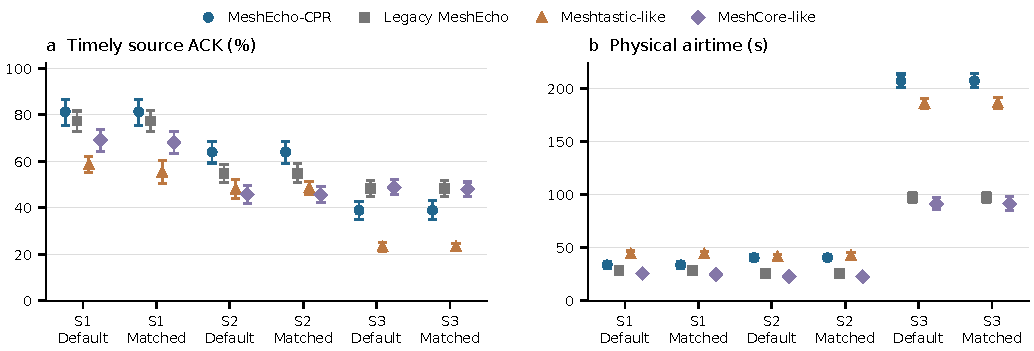
\includegraphics[width=\textwidth]{figures/formal-v2/main_results.pdf}
\caption{Complete main comparison. Points are equal-weight means of 20
seeds; bars are descriptive, unadjusted 95\% bootstrap intervals. Timely
ACK uses all scheduled flows; physical airtime includes all started frames.
The default and matched regimes are distinct cases, not 40 independent seeds.}
\label{fig:main-results}
\end{figure*}

\subsection{The trade-off changes with the operating condition}

Figure~\ref{fig:main-results} retains all four models and both regimes.
CPR's mean timely confirmation falls from 81.30\% in S1 to 63.96\% in S2
and 38.94\% in S3, while mean physical airtime increases from 33.79 to
40.55 and 207.07~s. Its resolved default and matched policies coincide.
The following paired contrasts use the matched regime; changes are
percentage points (pp), and bracketed bounds are descriptive 95\% intervals.

In S1, CPR exceeds legacy MeshEcho by 3.99~pp [$-1.61$, 9.08], with
an airtime ratio of 1.16 [1.06, 1.27]. This does not demonstrate a clear
confirmation improvement over legacy MeshEcho. Relative to Meshtastic-like,
CPR gains 25.99~pp [18.51, 33.31] at a ratio of 0.75 [0.70, 0.81]; relative
to MeshCore-like it gains 13.27~pp [8.04, 18.43] at 1.33 [1.20, 1.47].
These model comparisons include differing discovery and retry semantics.

In S2, CPR gains 9.28~pp [4.42, 14.00] over legacy MeshEcho, at a ratio
of 1.60 [1.50, 1.72]. Against Meshtastic-like the gain is 15.49~pp
[10.26, 20.74], with a ratio of 0.95 [0.91, 0.99]; against MeshCore-like
it is 18.41~pp [14.50, 22.33], with a ratio of 1.81 [1.69, 1.95]. Thus
improved confirmation need not mean reduced airtime.

The S3 result is adverse relative to both route-based comparators.
CPR loses 9.26~pp [$-14.13$, $-4.54$] against legacy MeshEcho and
9.04~pp [$-12.62$, $-4.88$] against MeshCore-like, while spending
2.13 [2.05, 2.24] and 2.29 [2.12, 2.46] times their airtime. It still
exceeds Meshtastic-like confirmation by 15.75~pp [12.25, 19.51], but at
an airtime ratio of 1.11 [1.09, 1.13]. Default-regime results preserve
these directions of the point estimates; parameter matching does not
remove the contention penalty.

\begin{table}[t]
\caption{Timely destination delivery (\%), matched regime. Equal-weight
20-seed means with descriptive 95\% intervals.}
\label{tab:delivery}
\centering\small
\setlength{\tabcolsep}{3pt}
\begin{tabular}{@{}lccc@{}}
\toprule
Model & S1 & S2 & S3 \\
\midrule
MeshEcho-CPR & 95.0 & 78.5 & 67.8 \\
 & [92.1, 97.1] & [75.7, 81.2] & [65.3, 70.2] \\
Legacy MeshEcho & 80.1 & 56.8 & 53.3 \\
 & [76.0, 84.1] & [52.6, 61.1] & [50.3, 56.3] \\
Meshtastic-like & 89.1 & 75.6 & 61.4 \\
 & [85.8, 92.0] & [72.4, 78.8] & [60.0, 62.7] \\
MeshCore-like & 72.8 & 48.7 & 53.4 \\
 & [68.3, 77.4] & [45.3, 52.5] & [50.4, 56.3] \\
\bottomrule
\end{tabular}
\end{table}

Delivery and confirmation diverge (Table~\ref{tab:delivery}). CPR has
67.81\% timely destination delivery in S3 despite only 38.94\%
confirmation. The corresponding legacy MeshEcho values are 53.29\%
and 48.20\%. Extra delivery alone therefore cannot establish the quality
of a confirmed transaction, and the gap does not by itself isolate the
cause of missing ACKs.

\subsection{Recovery helps disrupted paths and hurts under contention}

\begin{figure*}[t]
\centering
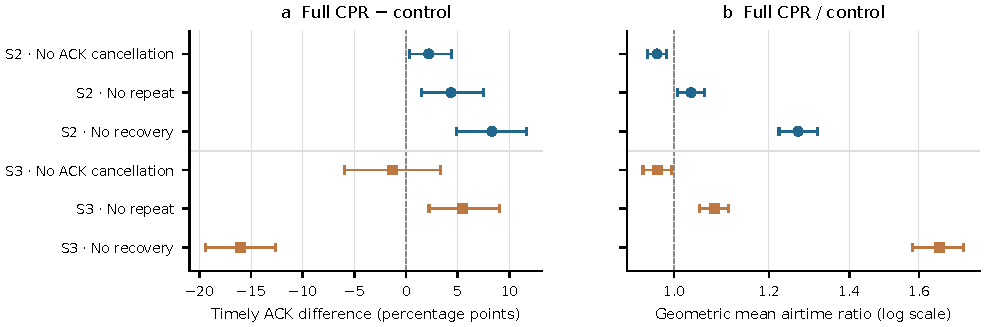
\includegraphics[width=\textwidth]{figures/formal-v2/component_effects.pdf}
\caption{Clean component controls in matched S2/S3, with all 20 paired
seeds. Panel (a) is full CPR minus the named control; panel (b) is the
geometric mean full/control physical-airtime ratio on a log scale.
Intervals are descriptive and unadjusted. Recovery's confirmation effect
reverses between the two settings.}
\label{fig:components}
\end{figure*}

Figure~\ref{fig:components} isolates each declared switch. In S2,
full CPR versus no recovery gains 8.32~pp [4.90, 11.63], at an airtime
ratio of 1.27 [1.22, 1.32]. In S3, the same contrast loses 15.99~pp
[$-19.41$, $-12.64$] and raises airtime to 1.66 [1.58, 1.74] times
that of the control. Removing recovery yields 54.93\% confirmation
and 125.21~s mean airtime, versus 38.94\% and 207.07~s for full CPR.
Its timely delivery is 64.94\%, versus 67.81\% for full CPR. Recovery
can therefore increase destination delivery while substantially harming
source confirmation in this contention setting.

The repeat contrast is positive in both settings: full versus no repeat
gains 4.35~pp [1.48, 7.51] in S2 and 5.43~pp [2.23, 9.01] in S3,
with airtime ratios 1.033 [1.007, 1.060] and 1.081 [1.051, 1.110].
The control preserves the nominal observation slot, so this comparison
includes the effects of removing the physical repeat and its downstream
contention while retaining the defined recovery timing rule.

ACK cancellation reduces paired airtime in S2 and S3: ratios are
0.968 [0.950, 0.986] and 0.968 [0.942, 0.995]. Its confirmation effect
is 2.20~pp [0.36, 4.38] in S2 but $-1.29$~pp [$-5.99$, 3.38] in
S3. The latter interval includes effects in both directions. These are
whole-policy paired costs, not savings inferred by multiplying canceled
copies by a nominal frame duration.

\subsection{Observed exposure and the boundary of mechanism evidence}

The complete S2 CPR population contains 648 scheduled flows per regime.
Among them, 85 routed initial transmissions start inside the fault window
with a carried path crossing a fault edge; each path had an accepted ACK
before the fault on the same generation. All 20 seeds expose this condition.
Of these 85 flows, 82 physically repeat and 78 start recovery; 24 deliver
on time, 18 receive a timely ACK, and 61 do not deliver on time. Every
successful first delivery and timely ACK in this subset is associated
with recovery marker 2. Twenty-three deliveries and 17 ACKs complete
within the active fault along avoiding paths. These stage associations
support mechanism interpretation; the no-recovery contrast supplies the
separate policy-effect evidence.

Across the full S2 population, 159 physical transmissions on fault edges
involve 87 flows: 78 initial DATA, 80 repeat DATA, and one ACK. None of
these intended receptions decodes. This population differs from the 85
initial-path crossings. Four of 25 fault-active flows whose initial send
precedes 80~s make a later actual fault-edge attempt. Exposure is measured
at physical TX start, without excluding cross-boundary failures or
unexposed scheduled flows from the main estimand.

S1 also exercises routed operation: per regime, 480 routed and 168
initial-flood starts serve the 648 flows; its 526 accepted ACKs traverse
four or six hops. S3 has 3059 scheduled flows, 2445 routed and 608
initial-flood starts, 1890 repeats, and 1597 recoveries. Intended-hop
capture-collision and half-duplex counts rise from 227/35 in S1 to
3228/887 in S3. These correlated hop/attempt outcomes indicate increased
contention, not independent flow failures. S3 has six source-state
capacity refusals and 52 protocol-no-start requests. Relay-ledger eviction
and capacity cancellation remain zero; peak ledger occupancy is not
reconstructed, so no measured memory-capacity advantage is claimed.

\subsection{Finite deadline and load response}

\begin{figure*}[t]
\centering
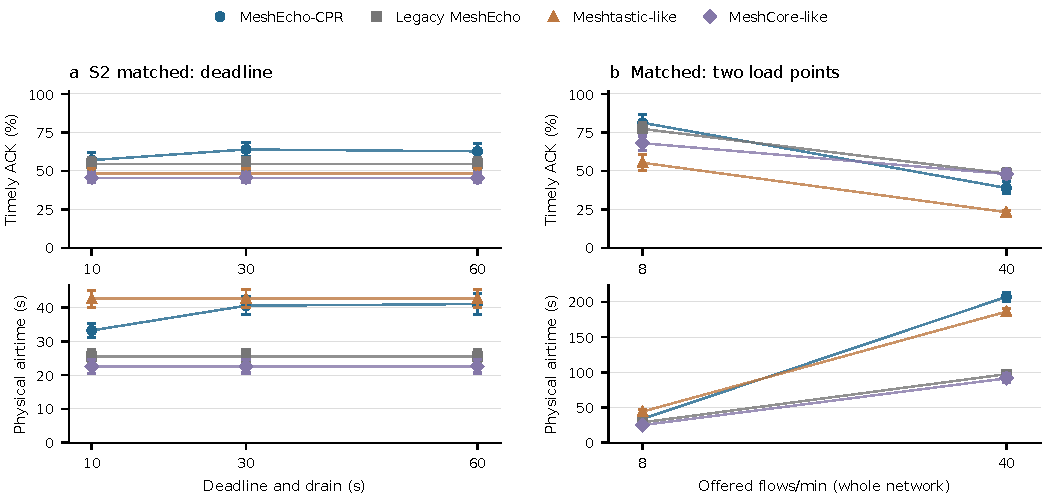
\includegraphics[width=\textwidth]{figures/formal-v2/robustness.pdf}
\caption{Prespecified finite response. (a) The S2 matched deadline axis
also changes drain duration; generation is always 240 s. (b) The two
fault-free offered loads reuse S1/S3 matched. Lines join observed points
only. All estimates use 20 seeds with descriptive 95\% intervals; no
cross-deadline inferential contrast or saturation threshold is claimed.}
\label{fig:robustness}
\end{figure*}

At deadlines of 10, 30, and 60~s, CPR's mean confirmation is 57.01\%,
63.96\%, and 62.74\%, with mean airtime 33.22, 40.55, and 41.05~s
(Fig.~\ref{fig:robustness}). The confirmation intervals are [51.75, 61.85],
[59.15, 68.57], and [57.32, 67.93]\%. There is no monotonic improvement
across all three points. Mean physical repeats per run are 6.3, 9.1, and
11.2; recovery starts are 0, 7.1, and 9.4. The 10-s case records 99
rejections specifically labeled \texttt{recovery-deadline-infeasible}.
Stale-route rejections are counted separately. Comparator point means
are unchanged across these three deadline/drain settings. The two load
points reproduce the S1/S3 reversal and do not locate its onset.

\subsection{Latency and physical-cost context}

\begin{figure*}[t]
\centering
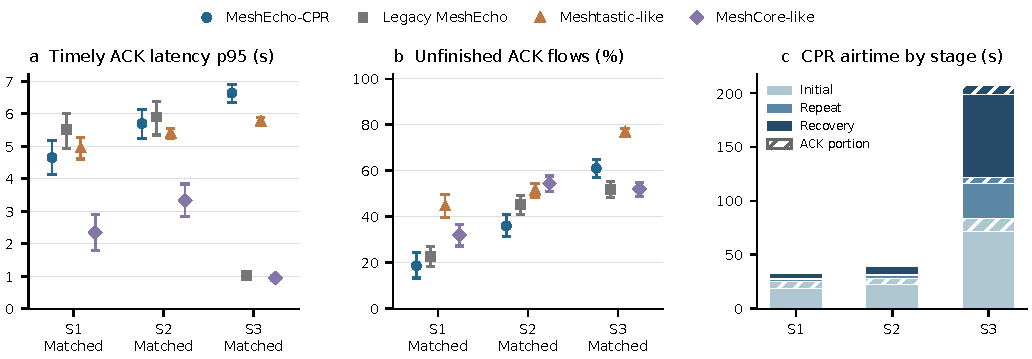
\includegraphics[width=\textwidth]{figures/formal-v2/latency_cost.pdf}
\caption{Matched main cases. (a) Mean of seed-level p95 latency among
timely ACK successes. (b) Unfinished ACK fraction over all scheduled
flows. (c) CPR physical airtime by source stage, including that stage's
relay traffic; hatching marks ACK airtime. Panels (a,b) show descriptive
95\% intervals; the additive cost partition shows means only.}
\label{fig:latency-cost}
\end{figure*}

The mean of CPR's seed-level timely-ACK latency p95 values is 4.65, 5.70,
and 6.63~s for S1/S2/S3 (Fig.~\ref{fig:latency-cost}). Its unfinished
ACK fractions are 18.70\%, 36.04\%, and 61.06\%. The short successful
latencies of the route-based comparators in S3 coexist with more than
half their flows lacking timely confirmation. Success-only latency is
therefore not a complete responsiveness ranking. CPR's mean airtime per
timely destination delivery rises from 1.11 to 1.61 and 2.01~s. The
stage partition reconstructs full physical airtime, including ACKs;
recovery occupies a large part of S3's cost. It neither measures device
energy nor assigns an independent confidence interval to each stacked
component.

\section{Discussion and Conclusion}
\label{sec:discussion}

The principal result is a boundary on fixed recovery: it improves timely
confirmation in the disrupted-path setting but worsens it under the
higher offered load. Local deadline feasibility is insufficient to decide
whether a recovery flood is beneficial to a shared channel. The clean
control reveals this limitation even though recovery-associated deliveries
exist and full CPR has higher destination delivery. Contention-aware
admission is a motivated future direction, not a policy evaluated here.

The external behavioral models omit documented retry and learning
behavior; custom frame lengths omit product framing and security overhead.
Parameter matching does not resolve these limits, so the results do not
establish product-firmware superiority. Twenty seeds, three scenarios,
and three deadlines provide finite descriptive evidence, not generality
across topology, traffic, and radio settings.

The radio model includes half-duplex operation, overlapping transmissions,
capture/interference decisions, and probabilistic reception, but has no
hardware calibration in this study. LoRa capture, imperfect spreading-factor
orthogonality, and aggregate interference can change real reception
behavior~\cite{rahmadhani2018concurrent,croce2018orthogonality,heusse2023capacity}.
The grid and fault fields are controlled stress settings. No duty-cycle or
listen-before-talk (LBT) enforcement is modeled. Fixed PHY, local timing,
and simplified queues leave device CAD timing, clock error, and application
diversity outside the claimed scope.
Transmit airtime does not measure whole-device energy or battery life.

Finite source stages and state limits do not guarantee delivery or bound
all simulator/firmware memory. Zero evictions do not measure peak ledger
occupancy. Canceled copies can change later contention, so their counts
alone do not establish network cost savings.

MeshEcho-CPR makes source-stage admission, route-evidence concurrency,
and the relay commitment boundary explicit. In the completed study,
same-path repeat improves confirmation in both tested component settings,
and ACK cancellation modestly reduces airtime. Recovery supplies a
conditional benefit with a substantial failure mode: its S2 gain of
8.32~pp becomes a 15.99-pp loss in S3. A useful recovery design must
therefore account for channel contention as well as remaining time.


\section*{Acknowledgment}
\textit{AI assistance.} OpenAI Codex assisted with literature organization,
drafting the abstract and Sections~\ref{sec:introduction}--\ref{sec:discussion},
the diagram and quantitative figure code, and development and verification
of the simulation and analysis software described in this paper. Its
outputs contributed manuscript text, code, and analysis explanations.

\bibliographystyle{IEEEtran}
\bibliography{references}
\end{document}
